\documentclass{article}
\usepackage{graphicx}
\usepackage{titletoc}
\usepackage{titlesec}
\usepackage{geometry} 
\usepackage{fontspec, xunicode, xltxtra}
\usepackage{float}
\usepackage{cite}
\usepackage{amsmath}
\usepackage{amssymb}
\usepackage{listings}
\usepackage{titletoc}
\usepackage{bm}

\geometry{left=3cm,right=3cm,top=3cm,bottom=3cm}
\DeclareMathOperator*{\argmin}{argmin}
\DeclareMathOperator*{\argmax}{argmax}
\DeclareMathOperator*{\var}{var}
\DeclareMathOperator*{\expec}{E}

\begin{document}
\title{\textsf{Homework 7 for Pattern Recognition}}
\author{Fan JIN\quad (2015011506)}
\maketitle

\section*{Question 1}
{
    \subsection*{Notations}
    {
        The multidimensional scaling (MDS) seeks to find a centered configuration $X = [x_1, \cdots, x_n]$, 
        where $x_1, \cdots, x_n \in \mathbb{R}^2$, 
        such that its distance matrix $\hat{D} = (\hat{d}_{ij}) \approx D$ where $$\hat{d}_{ij}^2 = (x_i - x_j)^T (x_i - x_j)$$ for $1 \leq i \leq n$ and $1 \leq j \leq n$.

        Define the Gram matrix $$B = (b_{ij}) = X^T X,$$ 
        and it follows that $$\hat{d}_{ij}^2 = x_i^T x_i + x_j^T x_j - 2 x_i^T x_j = b_{ii} + b_{jj} - 2 b_{ij}.$$

        By algebra manipulations\footnote{https://en.wikipedia.org/wiki/Multidimensional\_scaling}, 
        we can express $b_{ij}$ in terms of $d_{ij}$:
        $$\hat{B} = -\frac{1}{2} J \hat{D} J,$$
        where $$J = I_n - \frac{1}{n} 1 \cdot 1^T.$$

        Thus, we take $B$ as an estimate of $\hat{B}$, by reducing the dimension using the PCA approach. 
        Apply eigen decomposition and we obtain
        $$B = V * D * V^T,$$ where the eigenvalues are sorted in descending order.
        Retain the first two eigenvalues:
        $$\hat{B} = \hat{V} * \hat{D} * \hat{V}^T,$$
        where $\hat{V}$ is the first two columns of $V$, and $\hat{D}$ is the first two eigenvalues of the diagonal matrix $D$. Then, we have
        $$X = \hat{D}^{1/2} \hat{V}^T$$ which satisfies $$B = X^T X.$$
    }

    \subsection*{Visualization}
    {
        \begin{figure}[H]
            \centering
            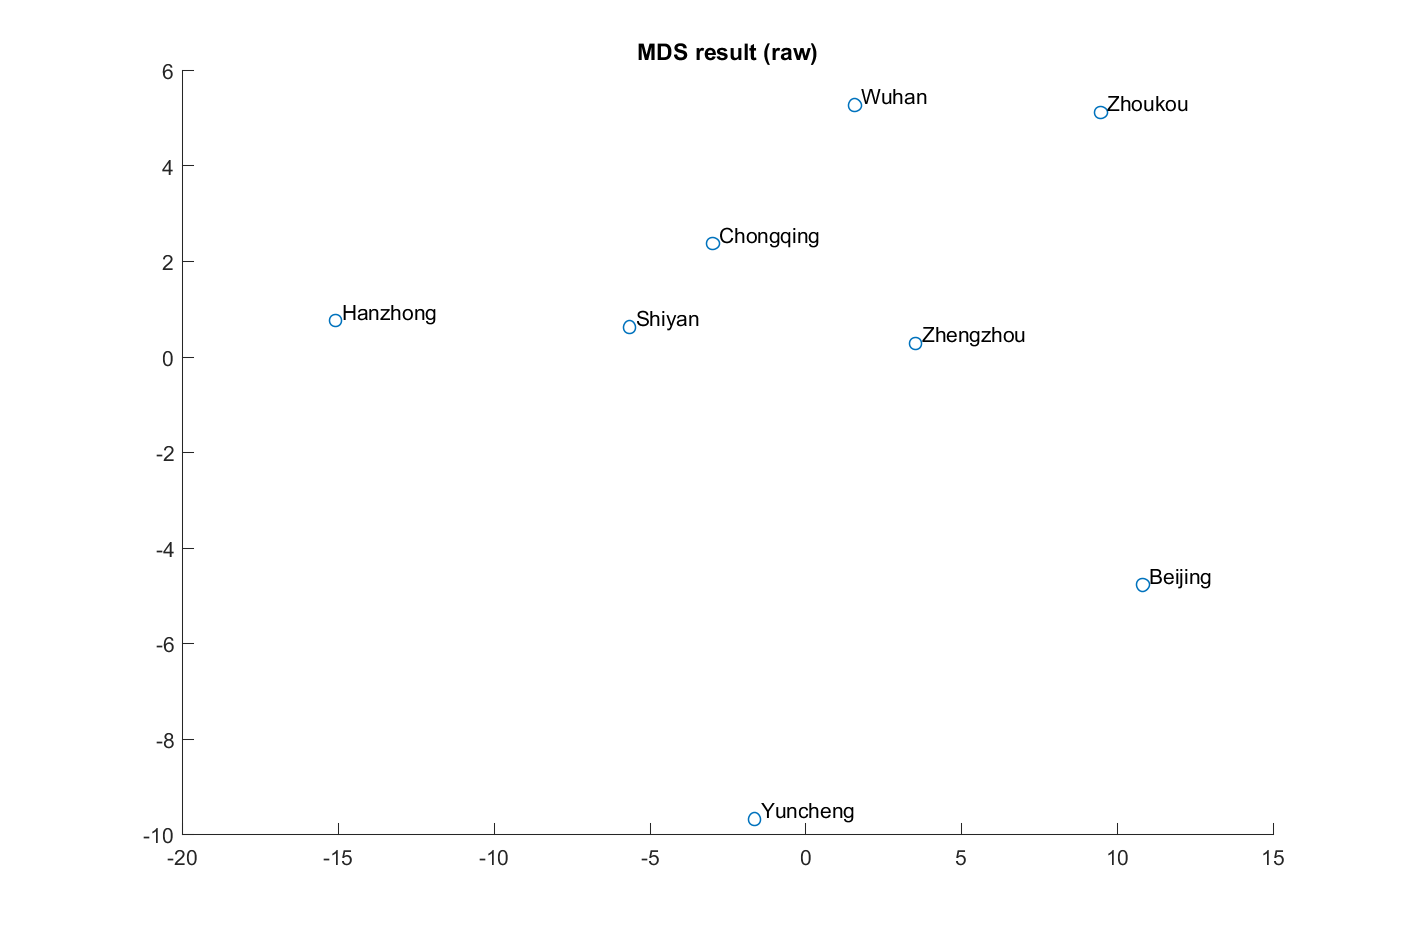
\includegraphics[width = 1\linewidth]{Q1/result.png}
            \caption{Raw result}
        \end{figure}

        To compare it with the actual satellite maps, we rotate it such that Zhengzhou is located roughly on the north of Wuhan.

        We see the cities in main lines (e.g. Beijing, Zhengzhou, Wuhan) preserve their relative location better, compared to those in branch lines. 
        This is mainly because the linearity between distance and traveling duration differs in the railway level. For main line railways, the traveling duration is usually linear with the distance on map, for they have
        \begin{itemize}
            \item routemaps much more straightforward,
            \item fewer stops,
            \item faster train speed.
        \end{itemize}

        It is noticed that the city Hanzhong seems like an outlier. This city, located in the middle of Mount Qinling and Mount Daba, was connected to other cities by a very slow branch line railway, before the construction of highspeed railways. This is why it is far away from other cities in the MDS map, although it is actually not so on the fringe.

        \begin{figure}[H]
            \centering
            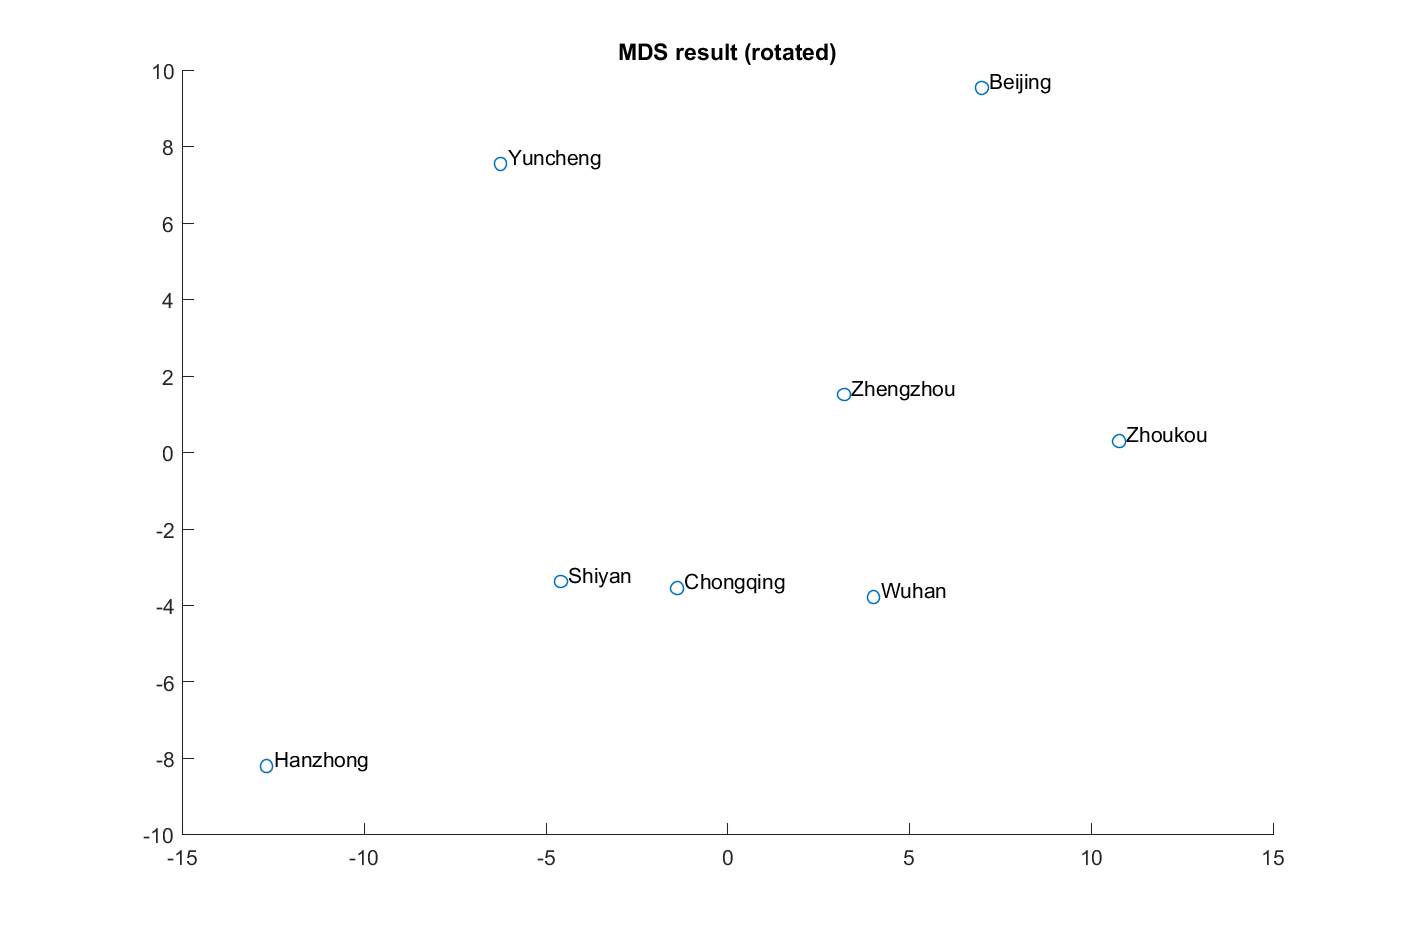
\includegraphics[width = 1\linewidth]{Q1/rotated.png}
            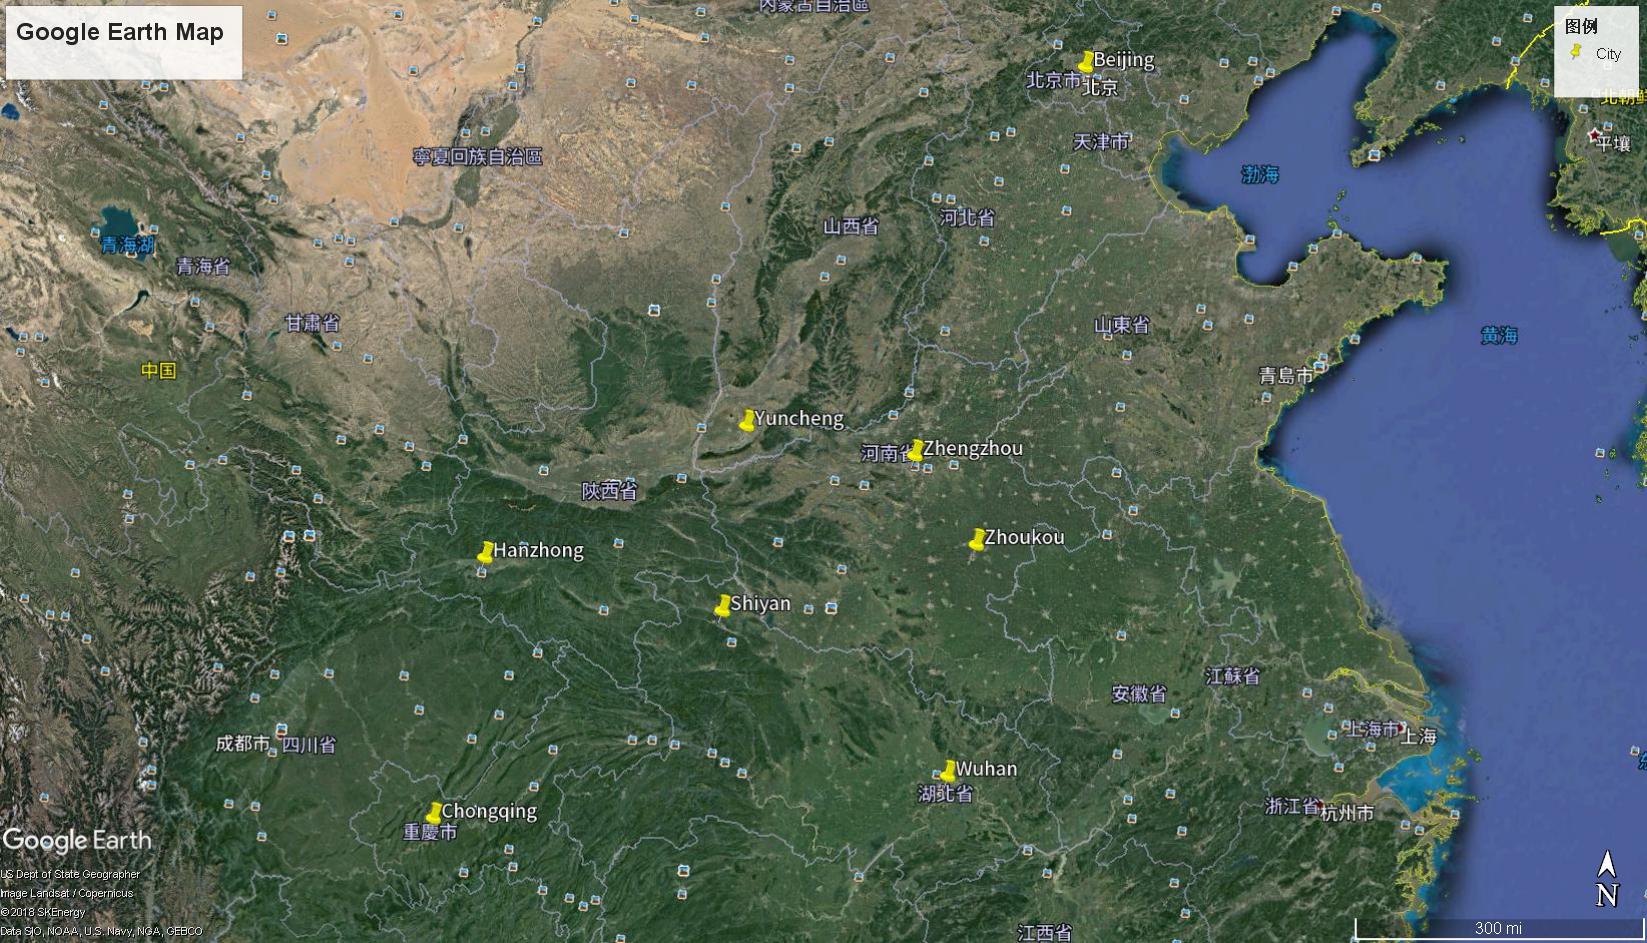
\includegraphics[width = 1\linewidth]{Q1/map.jpg}
            \caption{Comparison}
        \end{figure}
    }
}

\section*{Question 2a}
{
    \subsection*{PCA}
    {
        The PCA (principal component analysis) applies eigen decomposition to the covariance matrix (unnormalized) or correlation matrix (normalized) to the original data in $P$ dimensions, and only retains the first $p$ largest eigenvalues and their corresponding eigenvectors, which reconstructs the compressed data in $p$ dimensions. 
    }

    \subsection*{t-SNE}
    {
        The basic idea of t-SNE (t-distribution stochastic neighbor embedding) is to map the data to a probability distribution by affine transformation. 

        Given $N$ high dimensional objects $x_1, \cdots, x_N$, the t-SNE algorithm first computes a conditional probability, 
        which indicates the dissimilarity between two objects, 
        $$p_{j|i} = \frac{ \exp{(- \lVert x_i - x_j \rVert^2 / 2\sigma_i^2)} }{ \sum_{k\neq i} \exp{(- \lVert x_i - x_k \rVert^2 / 2\sigma_i^2)} },$$
        where the bandwidth of the Gaussian kernels $\sigma_i$ is set such that the perplexity of the conditional distribution equals a predefined perplexity. 
        This can be done using the bisection method. \footnote{https://en.wikipedia.org/wiki/T-distributed\_stochastic\_neighbor\_embedding}

        Given the conditional distributions, the joint distribution of two objects is computed as follows.
        $$p_{ij} = \frac{ p_{j|i} + p_{i|j} }{2N}.$$

        Unlike the classical SNE algorithm, the joint probabilities in low dimension space are computed in t-SNE using the t-distribution (heavy-tailed).
        $$q_{ij} = \frac{ (1 + \lVert y_i - y_j \rVert^2 )^{-1} }{ \sum_{k\neq i} (1 + \lVert y_i - y_j \rVert^2 )^{-1} }.$$

        The final step is to train the low dimensional objects $y_1, \cdots, y_N$ such that the KL distance below between the two distributions is minimized:
        $$\mathrm{KL}(P\Vert Q) = \sum_{i\neq j} p_{ij} \log{\frac{p_{ij}}{q_{ij}}}.$$

    }

    \subsection*{LLE}
    {
        The basic idea of LLE (locally linear embedding) is to map the data to a lower dimensional space while retaining the nonlinear manifold.
        \footnote{https://cs.nyu.edu/~roweis/lle/algorithm.html} 
        It hypothesize that each data point is a weighted linear combination of its neighboring objects, 
        and that such weights are shared in both original space and lower dimensional space. It consists of 3 steps:

        \begin{itemize}
            \item Calculate the $k$ nearest neighbors using KNN algorithms.

            \item Minimize the reconstruction loss
            $$\epsilon(W) = \sum_{i}{ \lVert X_i - \sum_{j}{W_{ij} X_j} \rVert ^2}$$
            subject to $$\sum_{j} {\frac{ \sum_k C_{jk}^{-1} }{ \sum_{lm} C_{lm}^{-1} }} = 1$$
            where the local convariance matrix $$C_{jk} = (x - \eta_j)^T (x - \eta_k)$$ with $\eta$ is the nearest neighbors of $x$.
        \end{itemize}

    }
}

\section*{Question 2b}
{
    \begin{figure}[H]
        \centering
        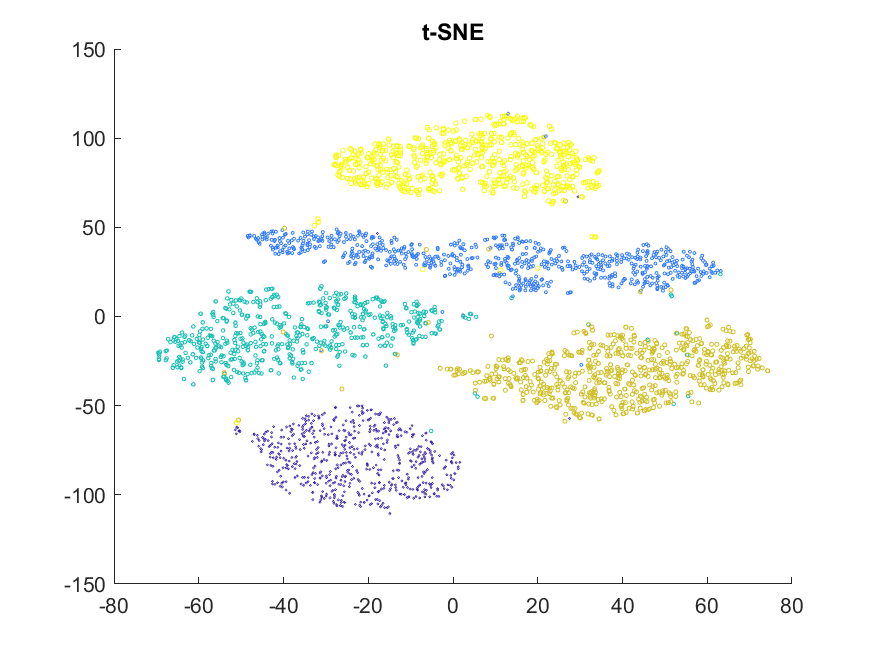
\includegraphics[width = 0.8\linewidth]{Q2/t-SNE.png}
        \caption{2D mapped data by t-SNE}
    \end{figure}

    \begin{figure}[H]
        \centering
        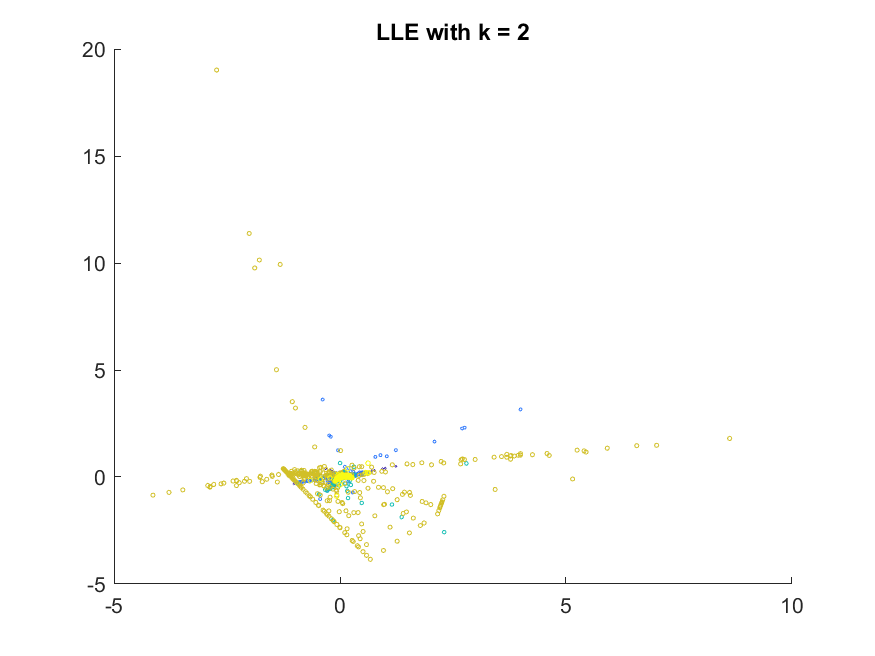
\includegraphics[width = 0.8\linewidth]{Q2/LLE_2.png}
        \caption{2D mapped data by LLE with k=2}
    \end{figure}

    \begin{figure}[H]
        \centering
        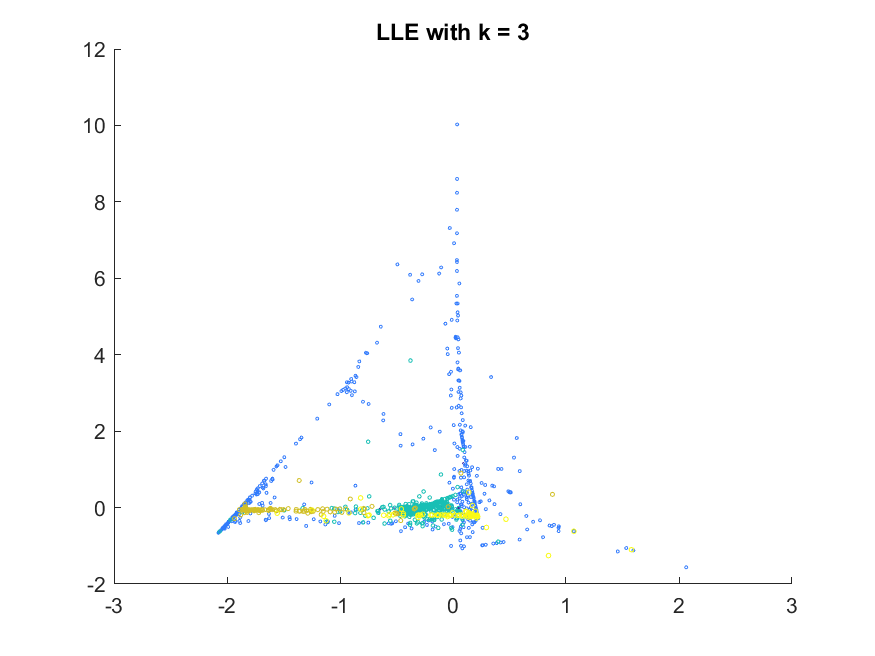
\includegraphics[width = 0.8\linewidth]{Q2/LLE_3.png}
        \caption{2D mapped data by LLE with k=3}
    \end{figure}

    \begin{figure}[H]
        \centering
        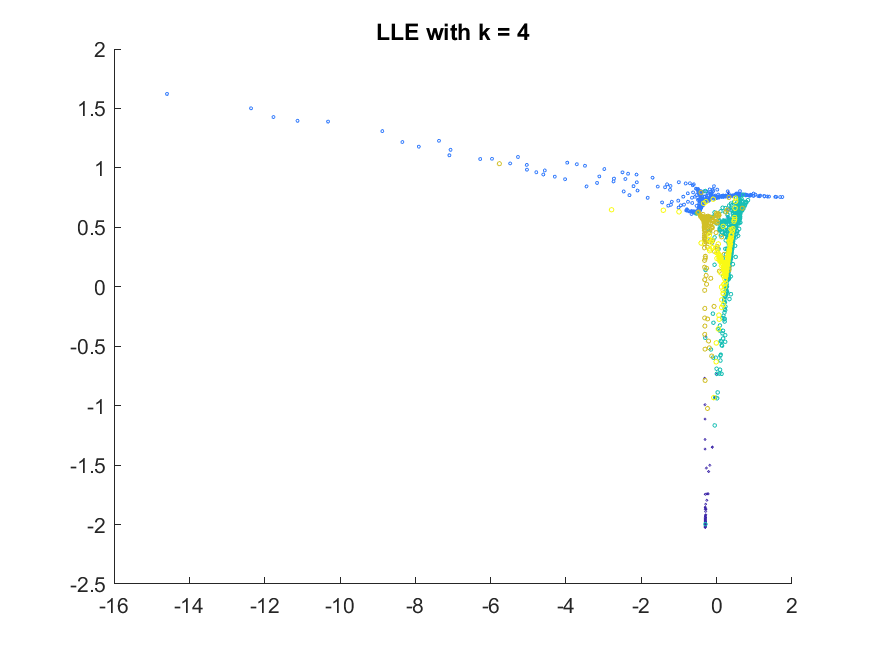
\includegraphics[width = 0.8\linewidth]{Q2/LLE_4.png}
        \caption{2D mapped data by LLE with k=4}
    \end{figure}

    \begin{figure}[H]
        \centering
        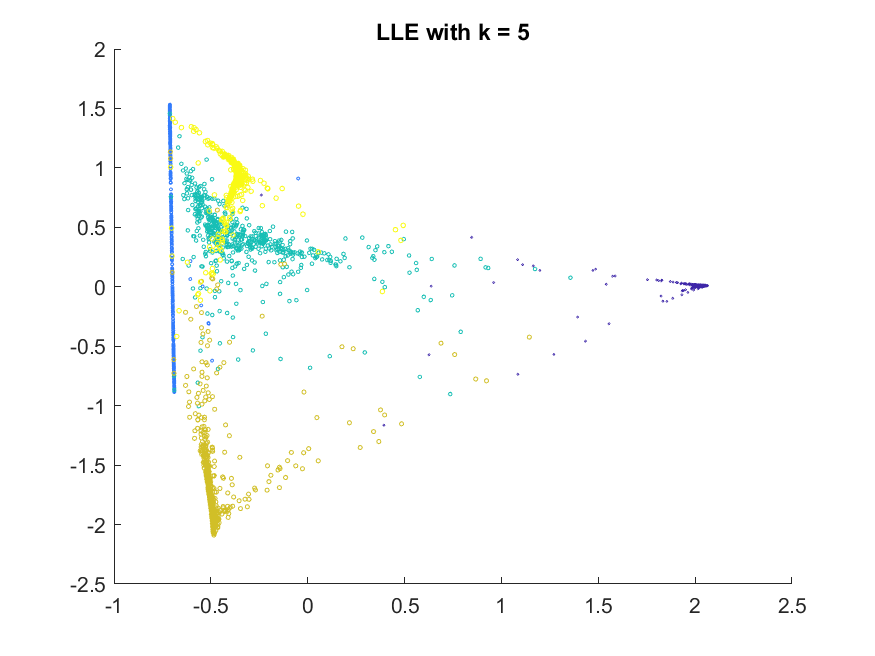
\includegraphics[width = 0.8\linewidth]{Q2/LLE_5.png}
        \caption{2D mapped data by LLE with k=5}
    \end{figure}

    \begin{figure}[H]
        \centering
        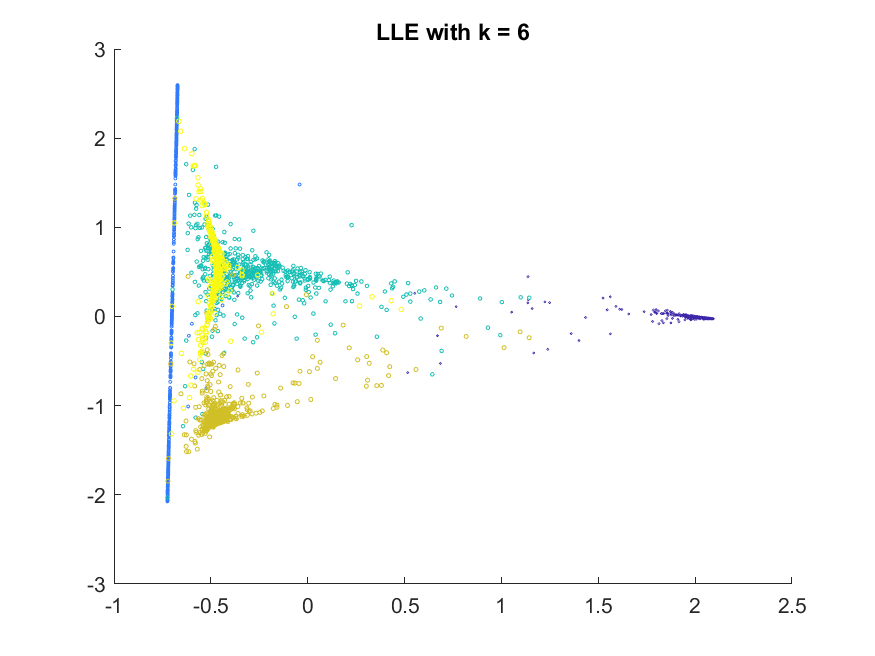
\includegraphics[width = 0.8\linewidth]{Q2/LLE_6.png}
        \caption{2D mapped data by LLE with k=6}
    \end{figure}

    \begin{figure}[H]
        \centering
        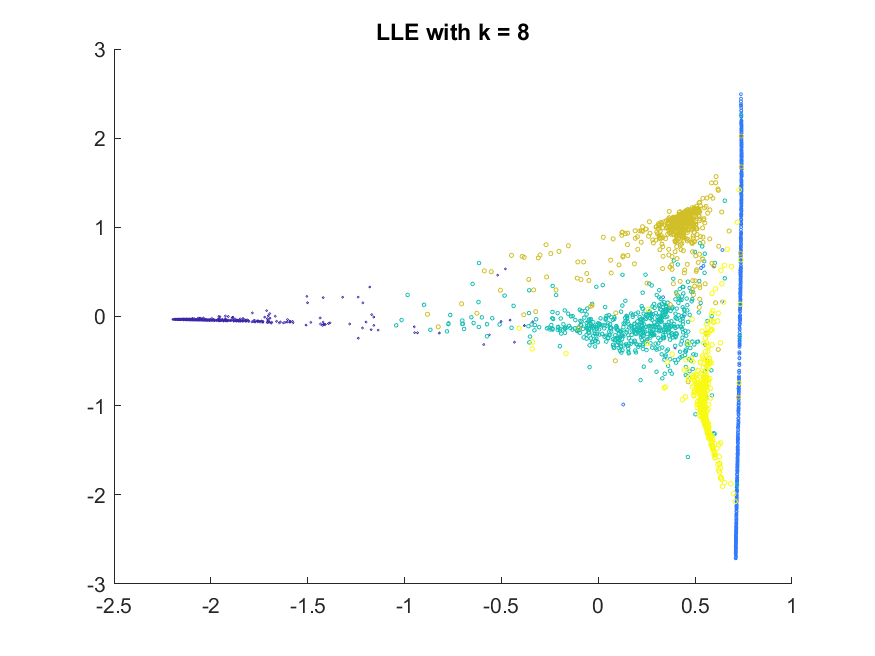
\includegraphics[width = 0.8\linewidth]{Q2/LLE_8.png}
        \caption{2D mapped data by LLE with k=8}
    \end{figure}

    \begin{figure}[H]
        \centering
        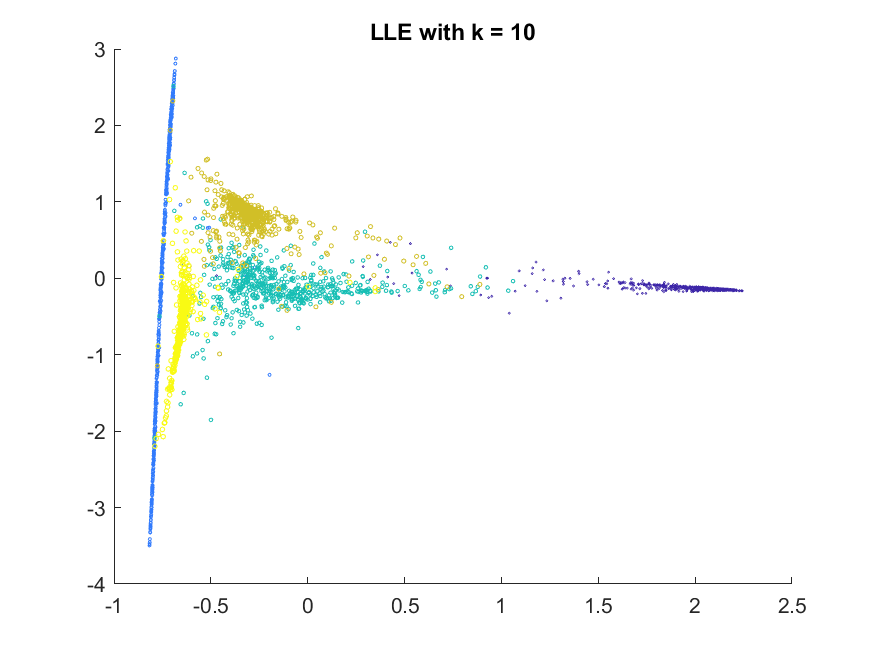
\includegraphics[width = 0.8\linewidth]{Q2/LLE_10.png}
        \caption{2D mapped data by LLE with k=10}
    \end{figure}

    \begin{figure}[H]
        \centering
        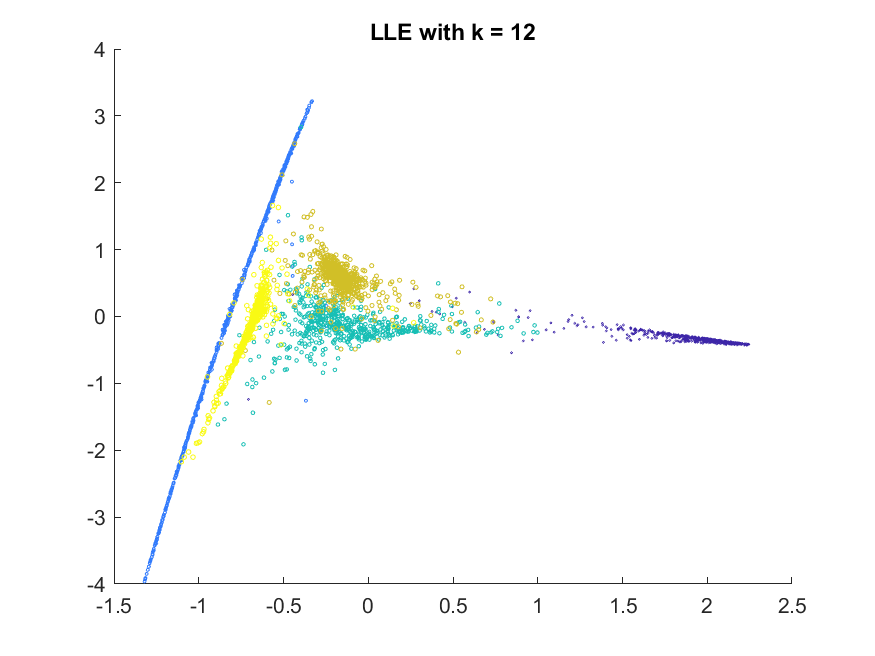
\includegraphics[width = 0.8\linewidth]{Q2/LLE_12.png}
        \caption{2D mapped data by LLE with k=12}
    \end{figure}

    \begin{figure}[H]
        \centering
        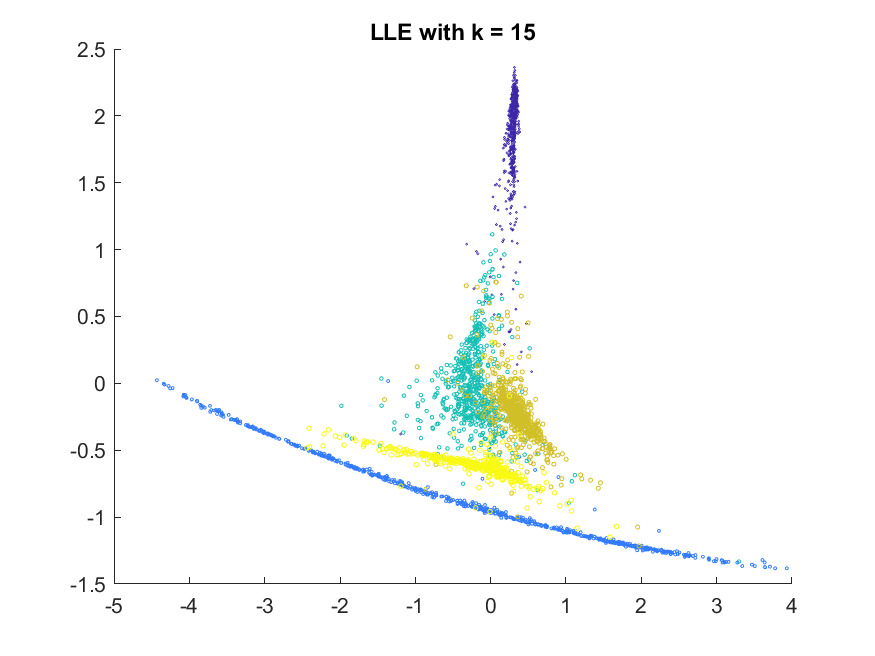
\includegraphics[width = 0.8\linewidth]{Q2/LLE_15.png}
        \caption{2D mapped data by LLE with k=15}
    \end{figure}

    \begin{figure}[H]
        \centering
        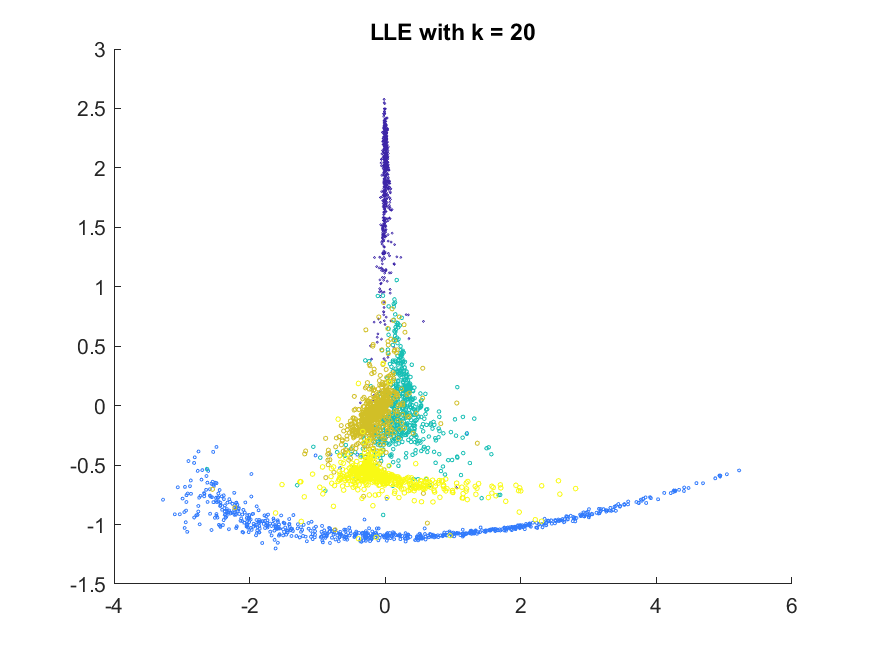
\includegraphics[width = 0.8\linewidth]{Q2/LLE_20.png}
        \caption{2D mapped data by LLE with k=20}
    \end{figure}

    \begin{figure}[H]
        \centering
        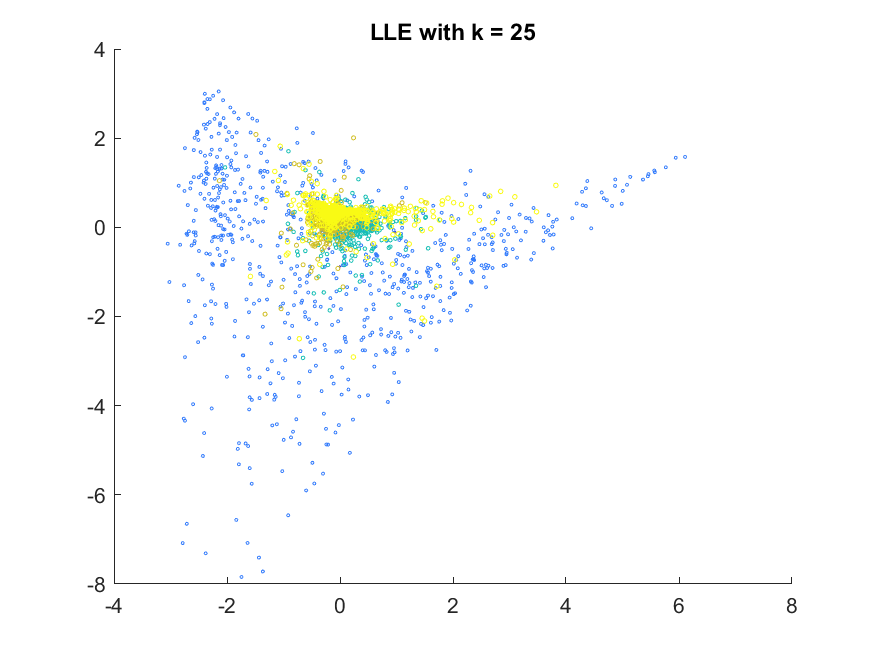
\includegraphics[width = 0.8\linewidth]{Q2/LLE_25.png}
        \caption{2D mapped data by LLE with k=25}
    \end{figure}

    \begin{figure}[H]
        \centering
        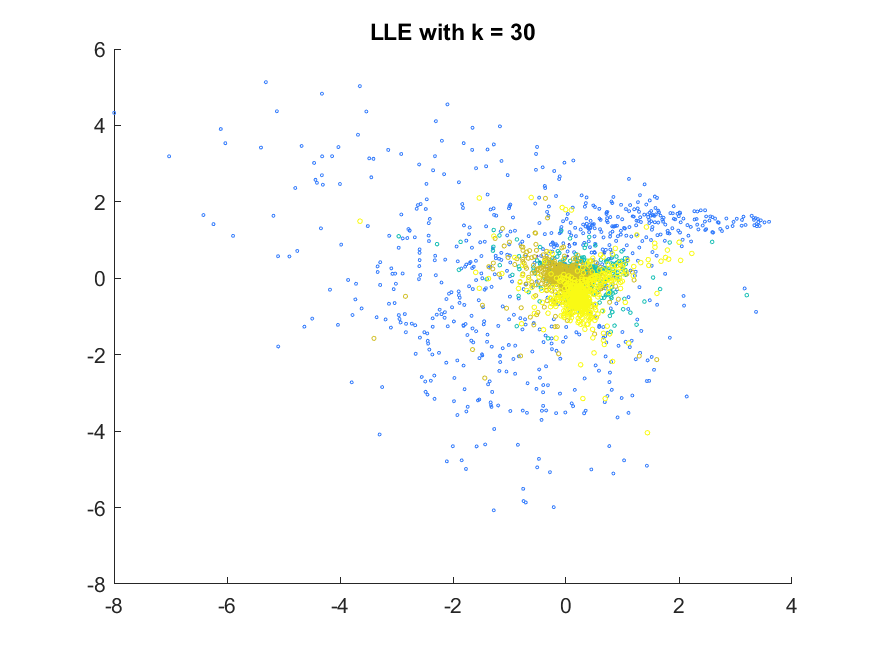
\includegraphics[width = 0.8\linewidth]{Q2/LLE_30.png}
        \caption{2D mapped data by LLE with k=30}
    \end{figure}

    \begin{figure}[H]
        \centering
        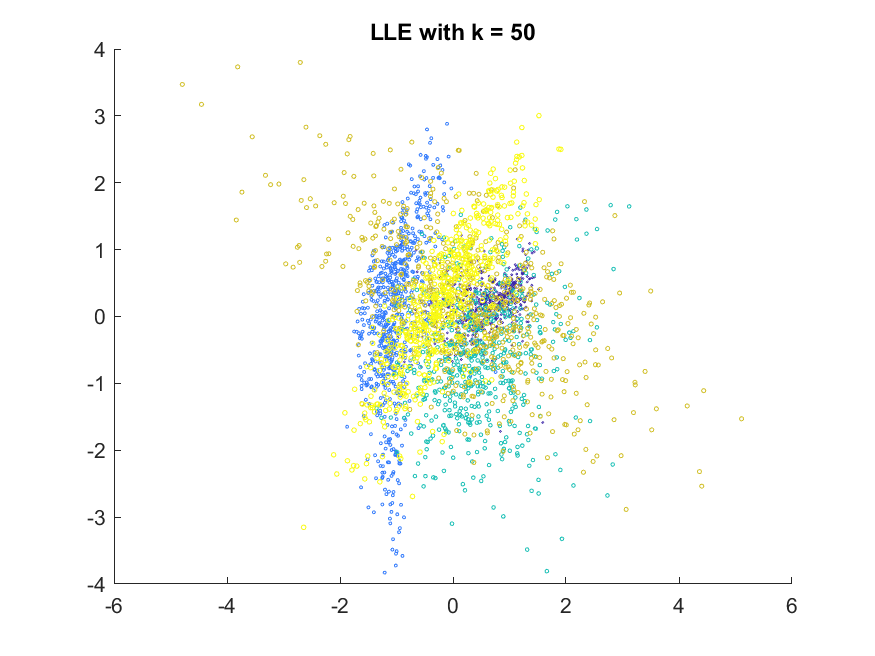
\includegraphics[width = 0.8\linewidth]{Q2/LLE_50.png}
        \caption{2D mapped data by LLE with k=50}
    \end{figure}
}

\section*{Question 2c}
{
    According to the author
    \footnote
    {
        Once I have a t-SNE map, how can I embed incoming test points in that map? \\
        t-SNE learns a non-parametric mapping, which means that it does not learn an explicit function that maps data from the input space to the map. 
        Therefore, it is not possible to embed test points in an existing map (although you could re-run t-SNE on the full dataset). 
        A potential approach to deal with this would be to train a multivariate regressor to predict the map location from the input data. 
        Alternatively, you could also make such a regressor minimize the t-SNE loss directly, which is what I did in this paper.
    },
    the incoming test points cannot be embedded in the t-SNE map. There are two workarounds.
    \begin{itemize}
        \item Re-run t-SNE on the full dataset. But the classifier we trained on training set would not work, since the re-run t-SNE map would differ from the previous one.
        \item Train a multivariate regressor to predict the map location.
    \end{itemize}

    In this project, we choose the latter workaround. We use the KNN classifier provided by the Classification Learner Toolbox in MATLAB. 
    And we achieve a testing accuracy of 0.983051 in the reduced model in 2 dimensional space, while it is 0.947034 in the full model in 784 dimensional space. 
}

\section*{Question 2d}
{
    In section 2b, we experimented the t-SNE algorithm, and the LLE algorithm with various hypermaramter $k$s. 

    \begin{itemize}
        \item The LLE requires a hyperparamter $k$, and the performance is quite sensitive to $k$. This means hypertuning is necessary, and a proper $k$ is crucial to the success.
        However, the output is separable within a range from $k=8$ to $k=20$. Many hypervalues are available for the algorithm.
        
        \item The t-SNE has no hyperparamters. But it has some weakness in that it is impossible to embed incoming test points to a pretrained map. 
        When a test point comes in, we have to re-train the model with the training set combined with the testing point, which is time consuming.
    \end{itemize}
}

\section*{Question 3}
{
    \begin{itemize}
        \item Classifier: Medium KNN (Classification Toolbox in MATLAB)
        \item Feature Selection by: KL Divergence
        \item Features to select from: 1000
        \item Validation: 10-fold
        \item Features to select: 20. We experimented from $p=2$ to $p=30$, and $p=20$ has the best performance in terms of validation accuracy.
    \end{itemize}

    The features selected are
    \begin{table}[!hbp]
        \centering
        \begin{tabular}{|c|c|c|c|c|}
        \hline
        361 & 425 & 662 & 166 & 219 \\
        \hline
        329 & 592 & 957 & 663 & 804 \\
        \hline
        542 & 817 & 395 & 281 & 778 \\
        \hline
        720 & 626 & 206 & 844 & 48 \\
        \hline
        \end{tabular}
        \caption{Features selected}
    \end{table}

    \begin{table}[!hbp]
        \centering
        \begin{tabular}{|c|c|c|}
        \hline
        & Full features & 20 selected features \\
        \hline
        Validation accuracy & 0.697500 & 0.797500 \\
        \hline
        \end{tabular}
        \caption{Comparison with 10-fold}
    \end{table}

    By feature selection with KL divergence, the accuracy of Medium KNN increases from 69.75\% to 79.75\%. What an improvement!
}

\section*{Source Code}
{
    Please download the souece code from http://39.106.23.58/files/PR7\_2015011506.7z

    For Question 2, please cd into ``Q1'' directory and run ``main.m''. 

    For Question 2, please cd into ``Q2'' directory run ``main.m''. It may take \emph{less than a minute} to train the network, but the result is reproducible because of the random seed.

    For Question 3, please cd into ``Q3'' directory run ``main.m''.

    For each model, I clicked ``Generate code'' button to transcript my operations into MATLAB codes, and stored each of them in the corresponding ``.m'' file. These files include:
    \begin{itemize}
        \item trainClassifierFull.m
        \item trainClassifierReduced.m
    \end{itemize}
    Thus, the steps above can be easily reproduced without using the GUI of the toolbox. 

}

\clearpage
\end{document}
    